\section{Experiments}\label{sec:exp}

\paragraph{Untuned baselines favor early triggering (Figure~\ref{fig:dose}).}
Against an uncertainty-blind current-gap rule and an unpadded current-margin rule, the $T_h=2.0$\,s predictive rule appears strong. With rate-limited recovery ($a_{\max}=1.0$), the uncertainty-blind rule fails first as fault severity grows, the unpadded rule collides in many moderate- and high-severity episodes, and the predictive rule records no collisions on this exploratory seed grid. This shows that earlier action can matter in the simulator, but not that prediction is needed; a padded current-margin rule can also act early.

\begin{figure}[tbp]
\centering
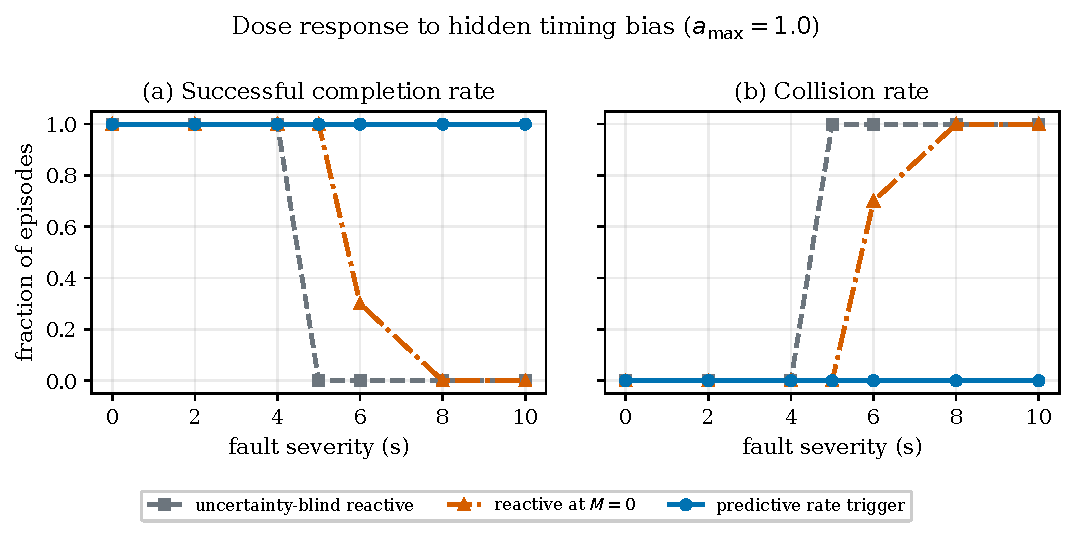
\includegraphics[width=\linewidth]{fig_dose.pdf}
\caption{Exploratory single-margin dose response with $T_h=2.0$\,s and rate-limited recovery. Results are observed rates over 40 paired noise seeds per severity. Figure~\ref{fig:boundary} adds an in-sample fixed-pad comparison.}
\label{fig:dose}
\end{figure}

\paragraph{Exploratory sweeps locate a narrow observed boundary (Figure~\ref{fig:boundary}).}
The plotted difference is the selected fixed-pad mean elapsed time minus the predictive mean, so positive values favor prediction. The fixed pad is selected in-sample at every setting. Under the slowest recovery ($a_{\max}=0.5$), the predictive rule finishes about $0.56$\,s sooner; the sign changes as recovery becomes faster, reaching $-1.31$\,s at $a_{\max}=3.0$. In the degradation-shape sweep at slow recovery, the predictor records collisions at $p=0.3$ and $p=0.5$, is about $1.23$\,s faster at $p=0.7$, and is slower than the selected fixed pad from $p=0.9$ onward. These differences are small relative to missions of roughly 25--30\,s, and the selection procedure does not support inferential claims.

\begin{figure}[tbp]
\centering
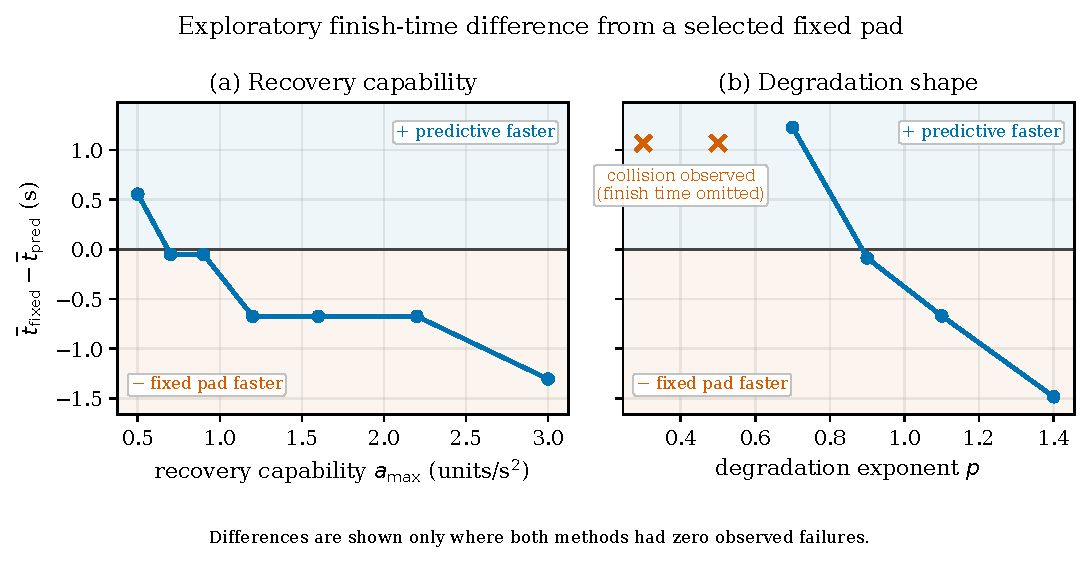
\includegraphics[width=\linewidth]{fig_boundary.pdf}
\caption{Exploratory elapsed-time difference between the $T_h=2.0$\,s predictive rule and the fixed pad selected on the same runs. Positive values favor prediction. Crosses replace timing comparisons where the predictive rule records a collision.}
\label{fig:boundary}
\end{figure}

\paragraph{Held-out tuning changes the comparison (Table~\ref{tab:heldout-single}).}
The finer, equal-budget searches select $\rho=2.5$ and $T_h=2.5$\,s. On the 6,750 held-out conflict episodes, the fixed rule succeeds in all 6,750 and records no collision. The tuned predictive rule succeeds in 6,748 and records two collisions, one at each of the two highest severities for $a_{\max}=0.5$ and $p=0.7$. Its successful-only mean elapsed time is $26.577$\,s, compared with $27.690$\,s for the fixed rule. These means condition on different success sets. Accordingly, we do not attach a paired interval or claim an efficiency advantage. For context, retaining the exploratory $T_h=2.0$\,s horizon on the same held-out conflict set gives 172 collisions in 6,750 episodes and 6,578 successful episodes; its successful-only mean is $25.990$\,s.

In the 2,250 held-out clear episodes, both tuned arms complete without collision. The fixed rule yields unnecessarily in $1800/2250$ episodes (80.0\%), while the predictive rule does so in $1358/2250$ (60.36\%). This is evidence of fewer interventions in the specified clear grid, not a safety-adjusted performance win. The maximum exact-scenario upper endpoint among the pointwise 95\% Wilson collision intervals is $0.0250$ for the fixed rule and $0.0368$ for the predictive rule. Taking the maximum does not turn those intervals into a simultaneous guarantee.

\begin{table}[tbp]
\centering
\small
\caption{Seed-disjoint single-margin test results. Elapsed time is averaged over successful conflict episodes only.}
\label{tab:heldout-single}
\begin{tabular}{lcccc}
\toprule
Arm & Parameter & Collisions & Successes & Mean time (s) \\
\midrule
Fixed margin & $\rho=2.5$ & $0/6750$ & $6750/6750$ & $27.690$ \\
Predictive, tuned & $T_h=2.5$ & $2/6750$ & $6748/6750$ & $26.577$ \\
Predictive, retained & $T_h=2.0$ & $172/6750$ & $6578/6750$ & $25.990$ \\
\bottomrule
\end{tabular}
\end{table}
